\documentclass[fleqn,10pt,serif,xcolor=svgnames,xcolor=table,aspectratio=169]{beamer}
% \includeonlyframes{current}
%========================================
% Packages
%========================================

\usepackage[palatino]{../99-auxiliary-files/00-mypackBeamer}
%========================================
% More Layout (Beamer Special)
%========================================

\DefineNamedColor{named}{mycol}{cmyk}{0.6,0.6,0,0}
% \DefineNamedColor{named}{mygray}{cmyk}{0.05,0.05,0.05,0.05}
% \DefineNamedColor{named}{mygraylight}{cmyk}{0.017,0.017,0.017,0.017}

\definecolor{signal1}{rgb}{0.69, 0.25, 0.21}
\definecolor{signal2}{rgb}{1.0, 0.66, 0.07}
\definecolor{signal3}{rgb}{0.39, 0.58, 0.93}
\definecolor{signal4}{rgb}{0.0, 0.4, 0.0}
\definecolor{firebrick}{rgb}{0.7, 0.13, 0.13}
\definecolor{themecolor}{rgb}{0.3, 0.36, 0.33} % feldgrau
\definecolor{darkgray}{rgb}{0.66, 0.66, 0.66}

% \usetheme[height=7mm]{Rochester}
%\usetheme{Warsaw}


\usecolortheme{dove}

% \useoutertheme[compress,subsection=false]{miniframes}

\usecolortheme[named=themecolor]{structure}

\setbeamercolor{title}{fg=themecolor}

% \setbeamercolor{lower separation line head}{bg=white}

%\setbeamercolor{structure}{fg=Brown}
%\setbeamercolor{normal text}{fg=Brown}
%\setbeamercolor{section in head/foot}{bg=gray!40}
%%\setbeamercolor{lower separation line head}{bg=black!40}
%\setbeamercolor*{frametitle}{fg=Black,bg=gray!40}
%\setbeamercolor*{block body}{fg=Brown,bg=gray!00}
%\setbeamercolor*{block title}{fg=Black,bg=gray!40}


% Switch of shadows of boxes
\setbeamertemplate{blocks}[default]

% Frame numbers in footer
\setbeamertemplate{footline}[frame number]

% See-through preview for uncovered
% \setbeamercovered{transparent}

% Switch off navigation panel at bottom right
\beamertemplatenavigationsymbolsempty

% Change Style for itemize markers
% Options are ball, circle, rectangle and default (=triangle)
\setbeamertemplate{items}[circle]



\setcounter{tocdepth}{1}

% Use bullets in enumerates and TOC
\setbeamertemplate{enumerate item}[circle]

% Set color for enumerate/TOC bullets to white
\setbeamercolor*{item projected}{fg=themecolor,bg=gray!00}

\setbeamercolor*{author}{fg=gray!80}

\setbeamerfont*{block title}{size=\normalsize}
\setbeamerfont*{title}{size=\huge}
\setbeamerfont*{subtitle}{size=\large}

% \newcommand{\mygray}[1]{{\color{gray}{#1}}}
% \newcommand{\mycol}[1]{{\color{mycol}{#1}}}

\newcommand{\mycomment}[1]{\hfill {\mygray{#1}}}
\newcommand{\mycom}[1]{\hfill {\mygray{[#1]}}}

\newcommand{\slideFN}[1]{%
  \begin{textblock*}{\paperwidth}(0pt,1.05\textheight)
    \hfill \footnotesize{\mygray{#1}} \hspace{.5em}
  \end{textblock*}}

\newcommand{\pictureslide}[2][current]{
\usebackgroundtemplate{\includegraphics[width=\paperwidth]{#2}}%
\begin{frame}[label=#1]

\end{frame}
}
% code below makes it possible to turn inclusion of frames
% into 'miniframes' off and on with commands:
% \miniframeson and \miniframesoff
% from: http://tex.stackexchange.com/questions/37127/how-to-remove-some-pages-from-the-navigation-bullets-in-beamer

\makeatletter
\let\beamer@writeslidentry@miniframeson=\beamer@writeslidentry
\def\beamer@writeslidentry@miniframesoff{%
  \expandafter\beamer@ifempty\expandafter{\beamer@framestartpage}{}% does not happen normally
  {%else
    % removed \addtocontents commands
    \clearpage\beamer@notesactions%
  }
}
\newcommand*{\miniframeson}{\let\beamer@writeslidentry=\beamer@writeslidentry@miniframeson}
\newcommand*{\miniframesoff}{\let\beamer@writeslidentry=\beamer@writeslidentry@miniframesoff}
\makeatother

\setbeamertemplate{bibliography item}{}

\usepackage{../99-auxiliary-files/00-mycommands}
\usepackage{array}
\usepackage[absolute,overlay]{textpos}

\usepackage{ulem}

% \usetheme[]{boxes}

%========================================
% Commands
%========================================

\newcommand{\mycol}[1]{{\textcolor{mycol}{#1}}}
\renewcommand{\markdef}[1]{\mycol{#1}}
\newcommand{\mygray}[1]{\textcolor{gray}{#1}}

\renewcommand{\slideFN}[1]{%
  \begin{textblock*}{\paperwidth}(0pt,0.95\textheight)
    \hfill \footnotesize{\mygray{#1}} \hspace{.5em}
  \end{textblock*}}

%========================================
% Document
%========================================

\title{Relations between \& operations on sets}
\subtitle{Methods: Logic, Part 1b}

\author{Michael Franke}
\date{}


%--------------------------------------

\begin{document}

% --- Horizontal Space Fix ----

\abovedisplayskip=3pt
\abovedisplayshortskip=3pt

\belowdisplayskip=3pt
\belowdisplayshortskip=3pt

\begin{frame}
  \maketitle
\end{frame}

\begin{frame}
  \frametitle{Content covered}

  \begin{itemize}
    \item relations between sets:
    \begin{itemize}
      \item (proper) subset
      \ (proper) superset
    \end{itemize}
    \item operations on sets:
    \begin{itemize}
      \item power set
      \item logical operations:
      \begin{itemize}
        \item intersection
        \item union
        \item difference
        \item complement
      \end{itemize}
    \end{itemize}
  \end{itemize}
\end{frame}

\begin{frame}
  \frametitle{Subsets}

  For any two sets $X$ and $Y$, $X$ is a \textbf{subset} of $Y$ if all elements of $X$ are also elements of $Y$. \\
  If $X$ is a subset of $Y$, we write: $X \subseteq Y$.\\
  If $X$ is not a subset of $Y$, we write: $X \not \subseteq Y$.

  \pause

\hfill  \textbf{Example 1: $A \subseteq B$}

  \hfill 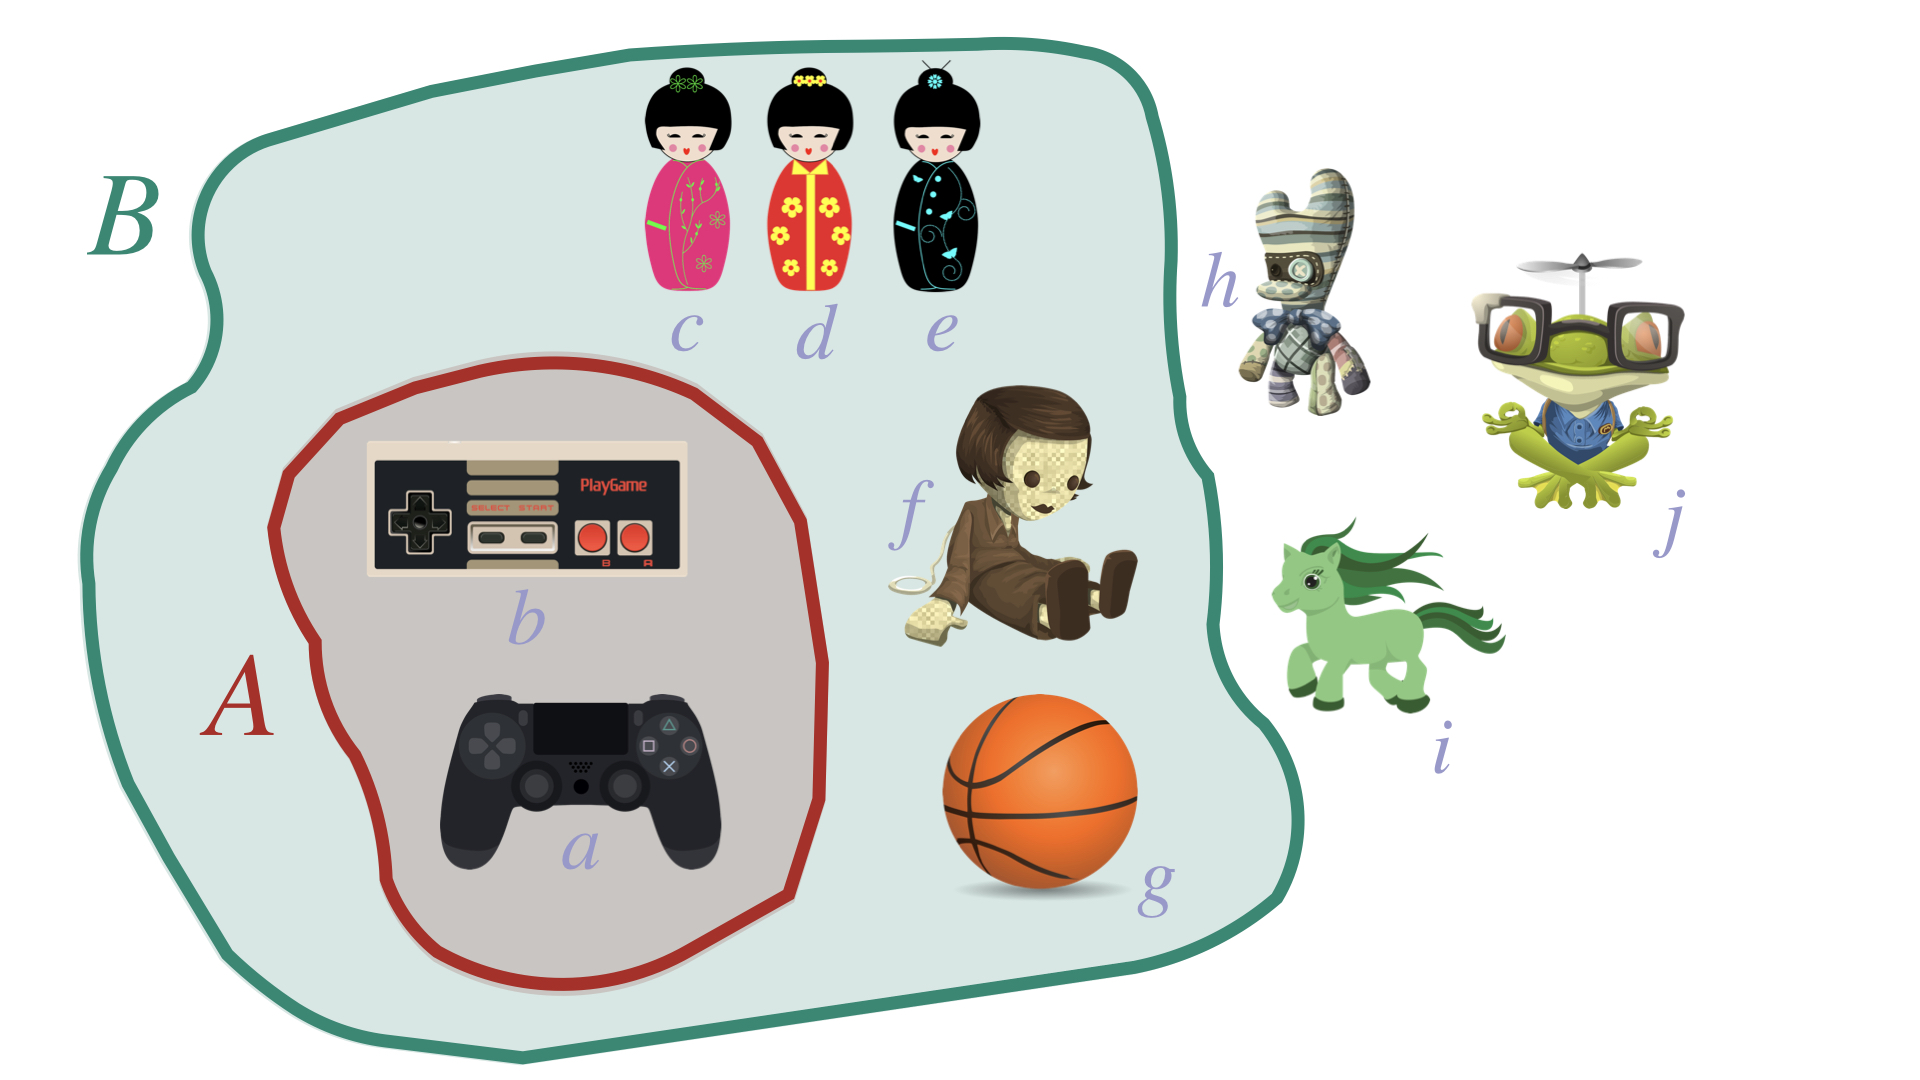
\includegraphics[width = 0.7\textwidth]{01b-sets-relations-operations/01b-sets-relations-operations-001.jpeg}

\end{frame}

\begin{frame}
  \frametitle{Subsets}

  For any two sets $X$ and $Y$, $X$ is a \textbf{subset} of $Y$ if all elements of $X$ are also elements of $Y$. \\
  If $X$ is a subset of $Y$, we write: $X \subseteq Y$.\\
  If $X$ is not a subset of $Y$, we write: $X \not \subseteq Y$.

  \bigskip

  \hfill \textbf{Example 2: $C \not \subseteq B$}

  \hfill 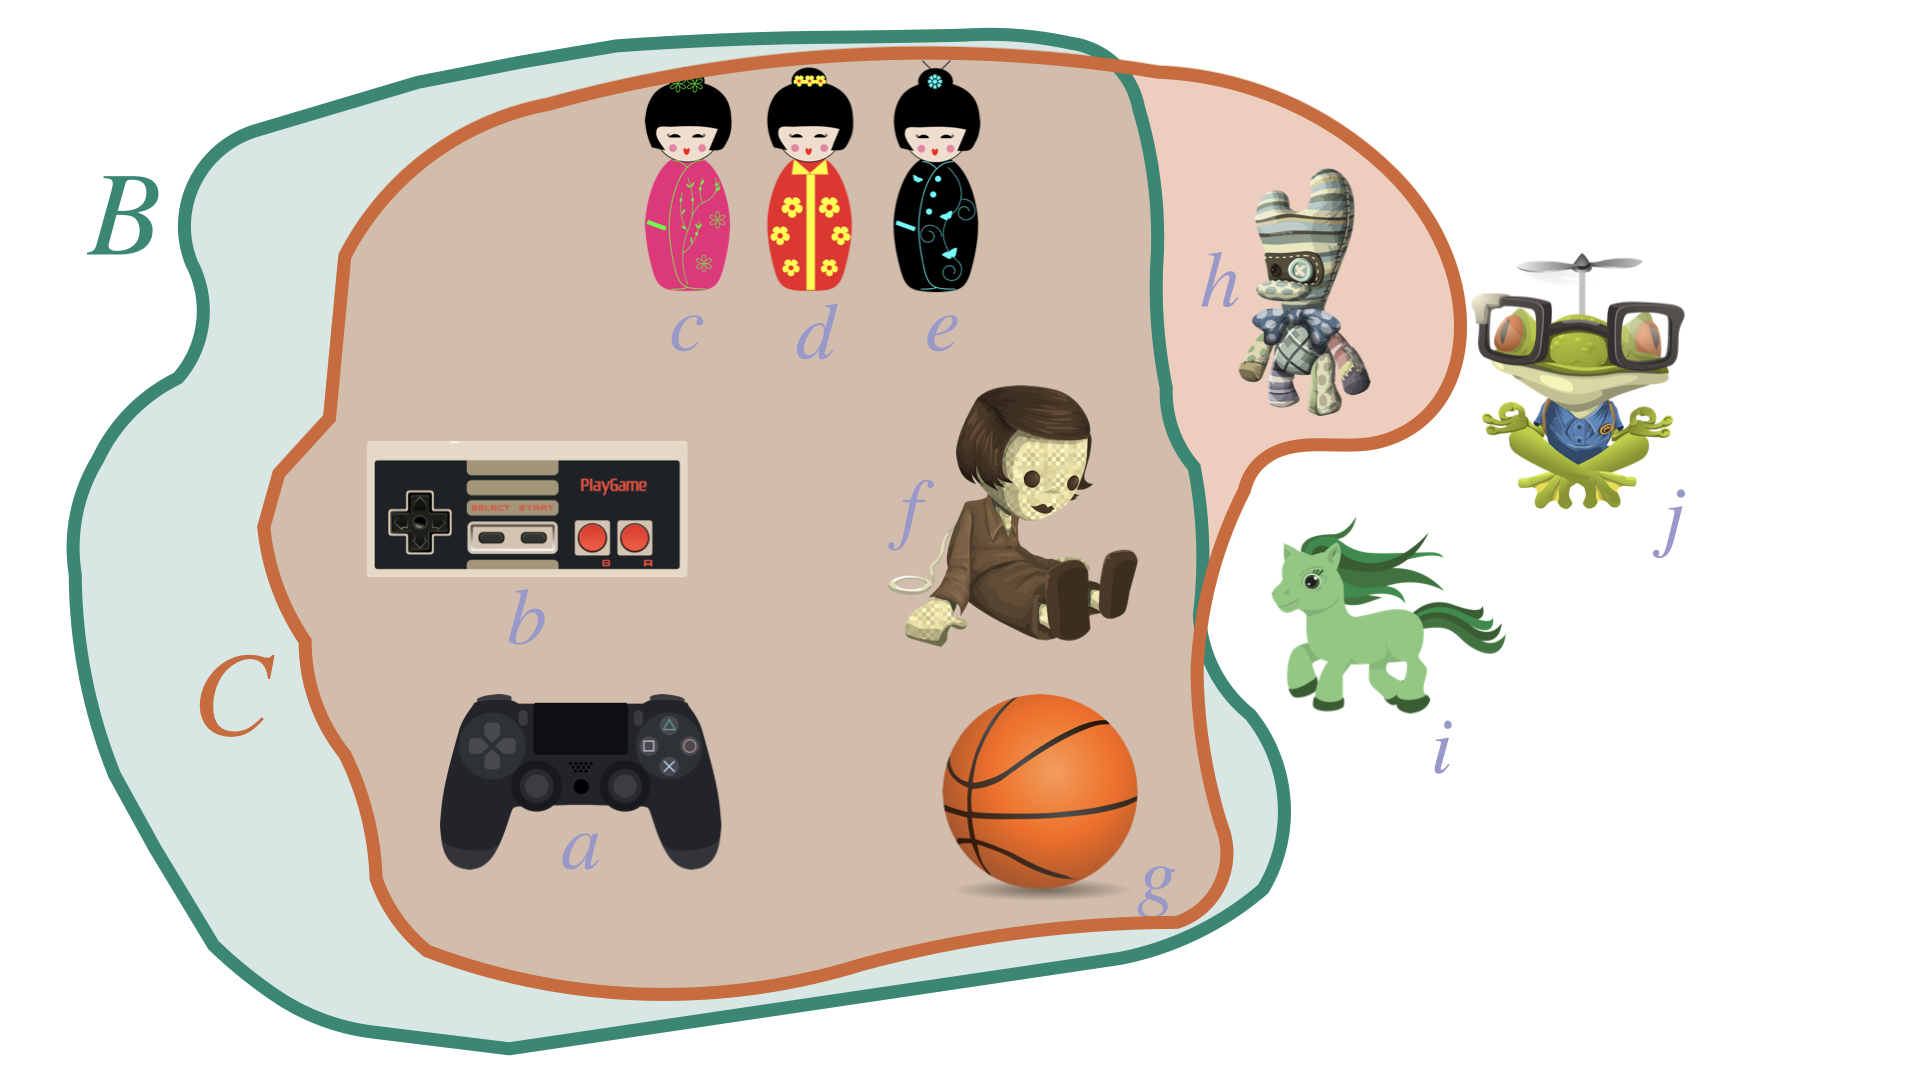
\includegraphics[width = 0.7\textwidth]{01b-sets-relations-operations/01b-sets-relations-operations-002.jpeg}

\end{frame}

\begin{frame}
  \frametitle{Proper subsets}

  For any two sets $X$ and $Y$, $X$ is a \textbf{proper subset} of $Y$ if all elements of $X$ are also elements of $Y$ and there is at least one element $y \in Y$ such that $y \not \in Y$.\\
  If $X$ is a proper subset of $Y$, we write: $X \subset Y$.\\
  If $X$ is not a proper subset of $Y$, we write: $X \not \subset Y$.

\pause

  \bigskip

  \hfill \textbf{Example 3: $A \subset B$}

  \hfill 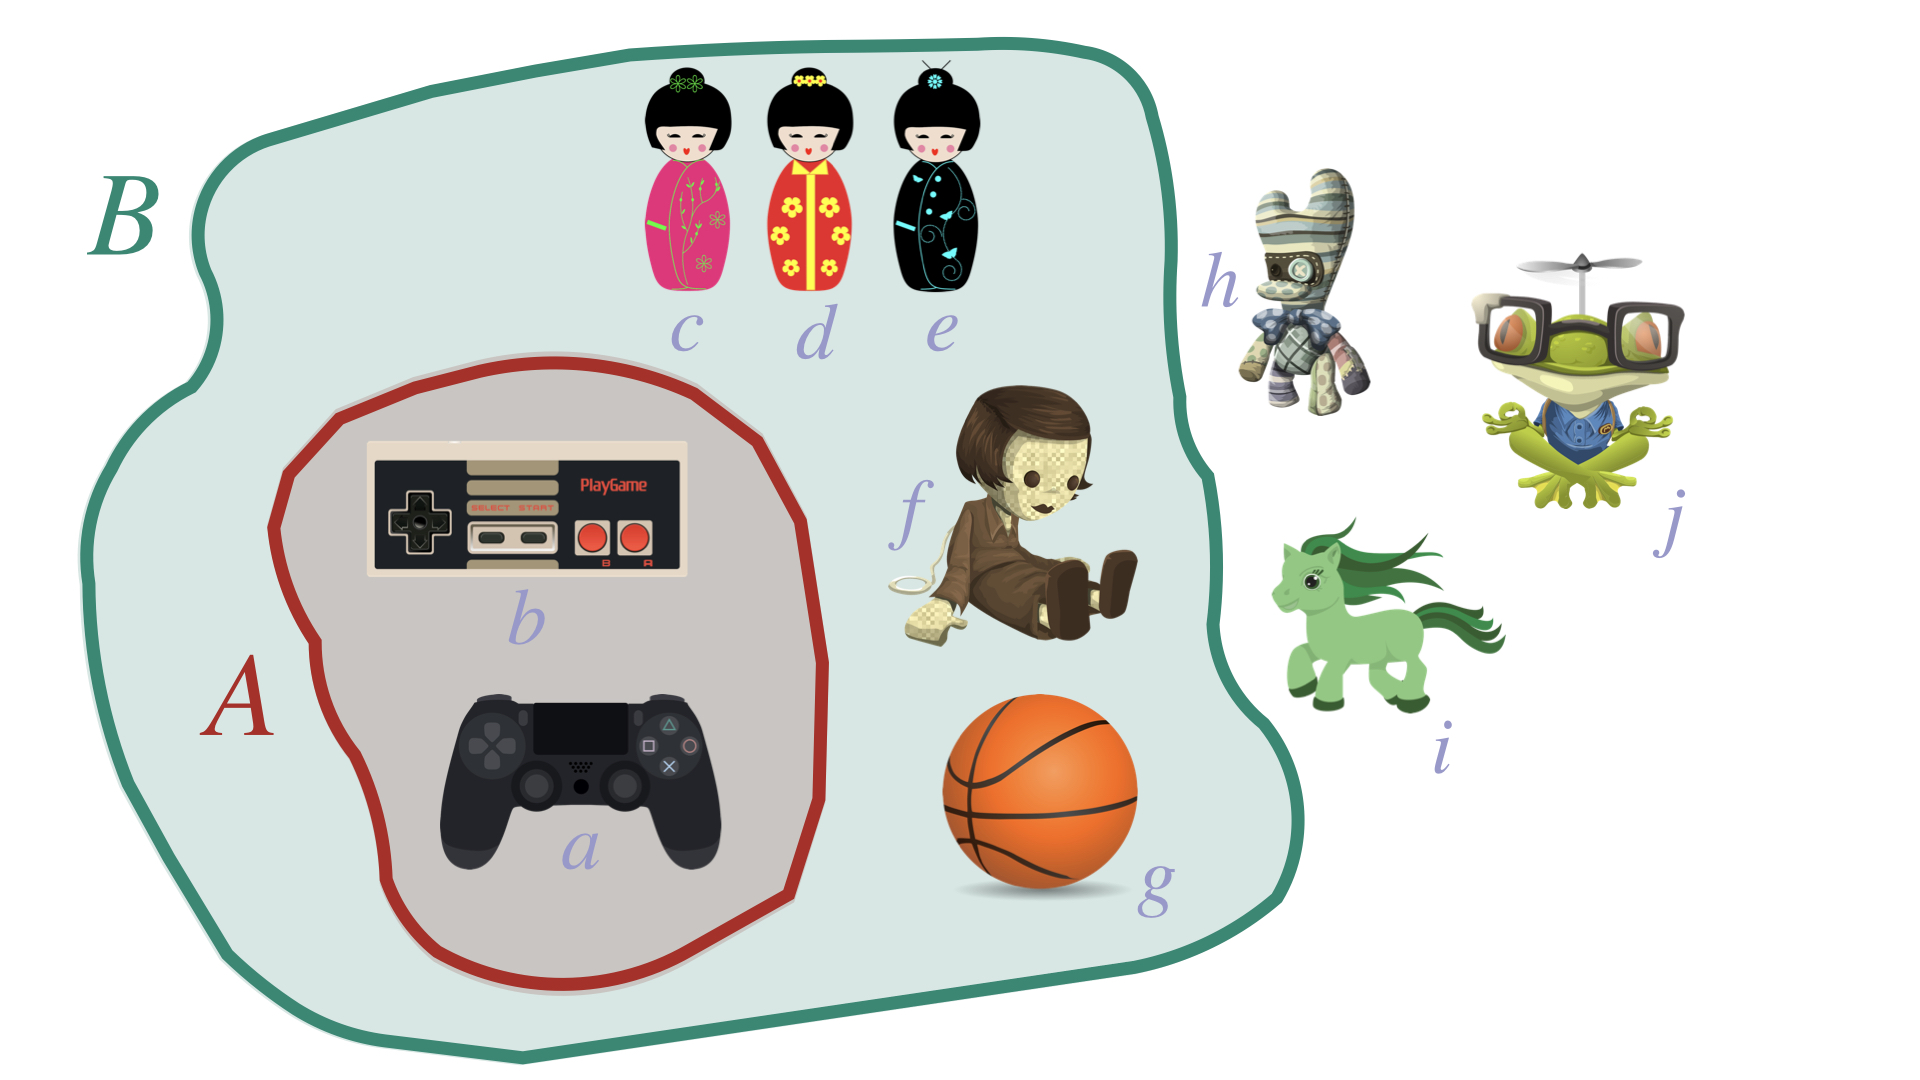
\includegraphics[width = 0.7\textwidth]{01b-sets-relations-operations/01b-sets-relations-operations-001.jpeg}

\end{frame}

\begin{frame}
  \frametitle{Proper subsets}

  For any two sets $X$ and $Y$, $X$ is a \textbf{proper subset} of $Y$ if all elements of $X$ are also elements of $Y$ and there is at least one element $y \in Y$ such that $y \not \in Y$.\\
  If $X$ is a proper subset of $Y$, we write: $X \subset Y$.\\
  If $X$ is not a proper subset of $Y$, we write: $X \not \subset Y$.



  \hfill \textbf{Example 4: $B \not \subset B$ (but $B \subseteq B$)}

  \hfill 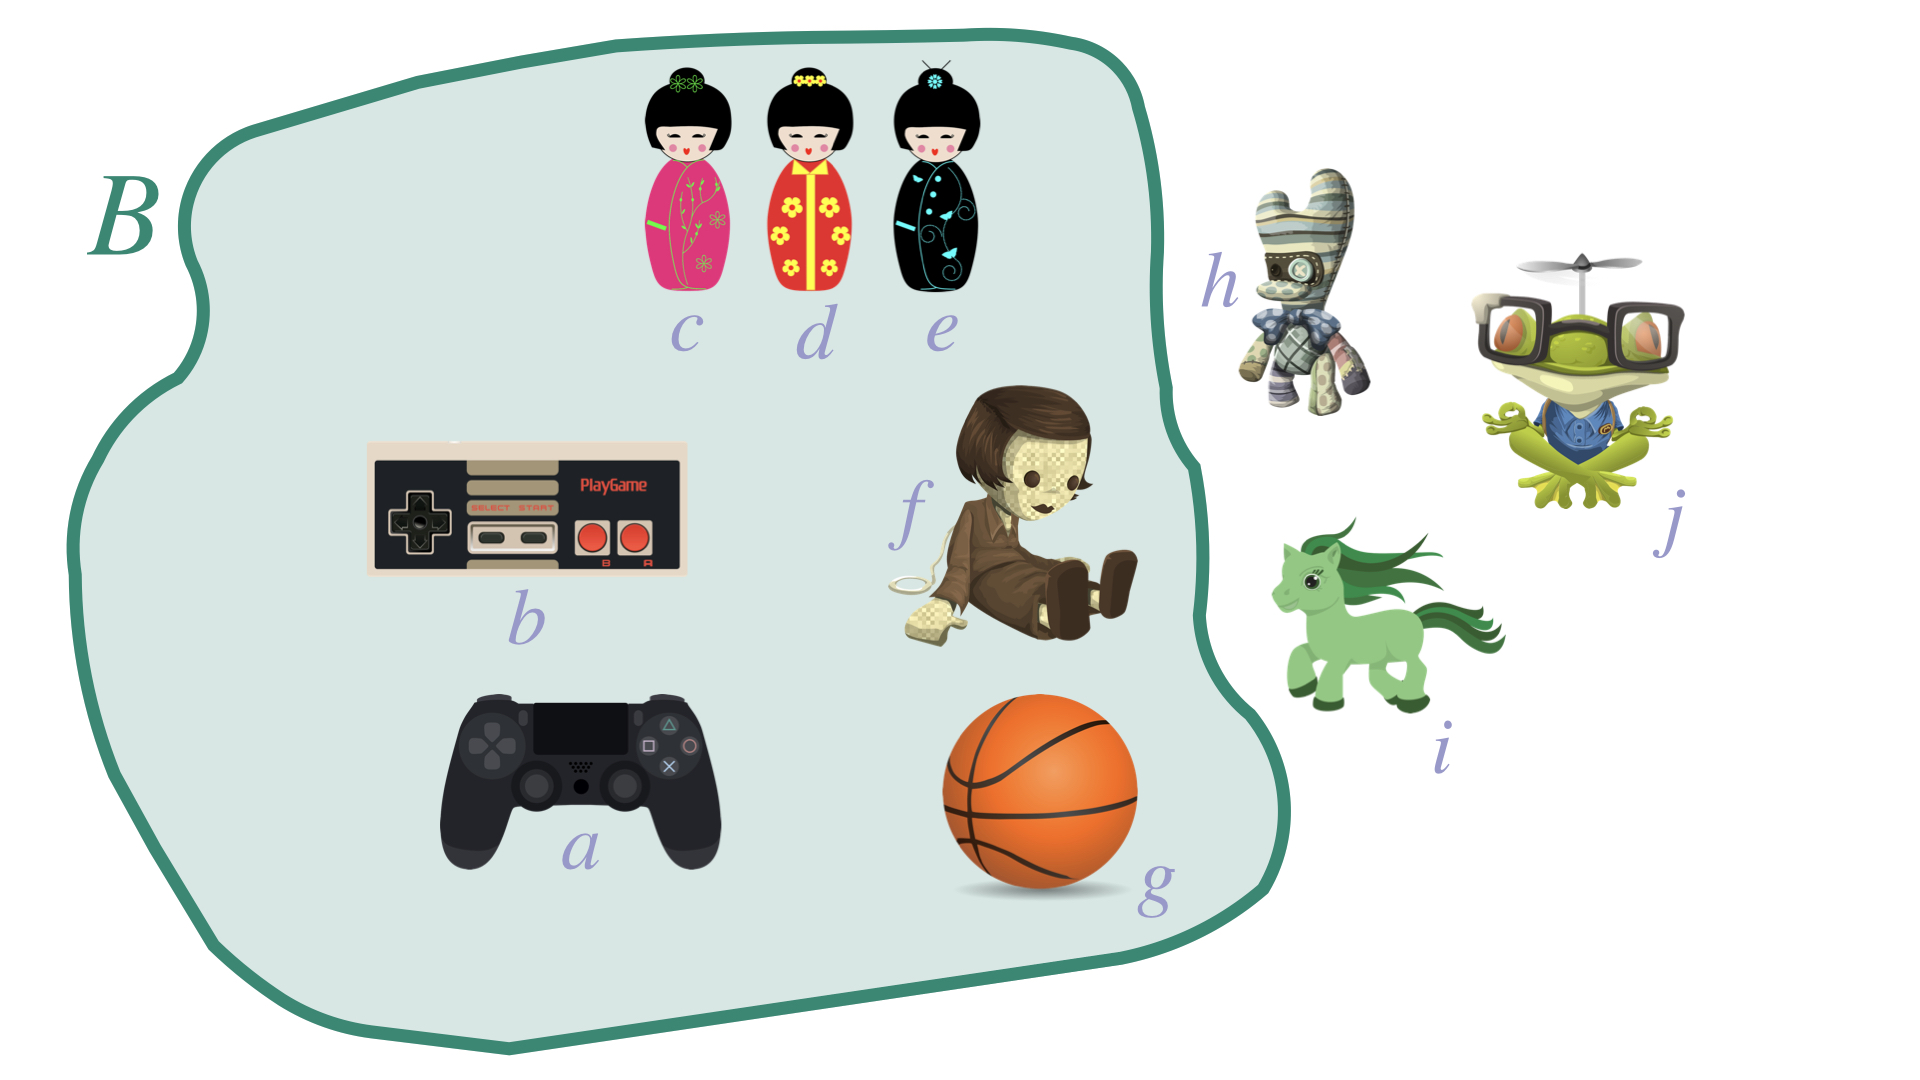
\includegraphics[width = 0.7\textwidth]{01b-sets-relations-operations/01b-sets-relations-operations-003.jpeg}

\end{frame}

\begin{frame}
  \frametitle{Superset and proper supersets}
  If $X$ is a (proper) subset of $Y$, then $Y$ is a \textbf{(proper) superset} of $X$.\\
  If $Y$ is a superset of $X$, we write: $X \subseteq Y$ or $Y \supseteq X$.
\end{frame}

\begin{frame}

\frametitle{Power set}

  The \textbf{power set} $\pow{X}$ of $X$ is the set of all subsets of $X$:
  \begin{align*}
    \pow{X} = \set{Y \setbar Y \subseteq X}
  \end{align*}

  \bigskip

  \textbf{Example 5}:

    \begin{enumerate}[]
      \item $X = \set{a,b}$
      \item $\pow{X} = \set{\emptyset, \set{a}, \set{b}, \set{a,b}}$
    \end{enumerate}

\end{frame}

\begin{frame}
  \frametitle{Logical operations on sets}
\begin{enumerate}[]
\item $X \cap Y = \set{z \setbar z \in X \text{ and } z \in Y}$ \hfill \mygray{[intersection]}
\item $X \cup Y = \set{z \setbar z \in X \text{ or } z \in Y}$ \hfill \mygray{[union]}
\item $X \setminus Y = \set{z \setbar z \in X \text{ and } z \not \in Y}$ \hfill
  \mygray{[difference]}
\item $\overline{X} = \set{z \in U \setbar z \not \in X }$ \hfill
  \mygray{[complement]}
\end{enumerate}

\end{frame}

\begin{frame}
  \frametitle{Example: Intersection}

  \hfill \textbf{Example 6: $B \cap C = \set{a, b , \dots, g}$}

  \bigskip

  \hfill 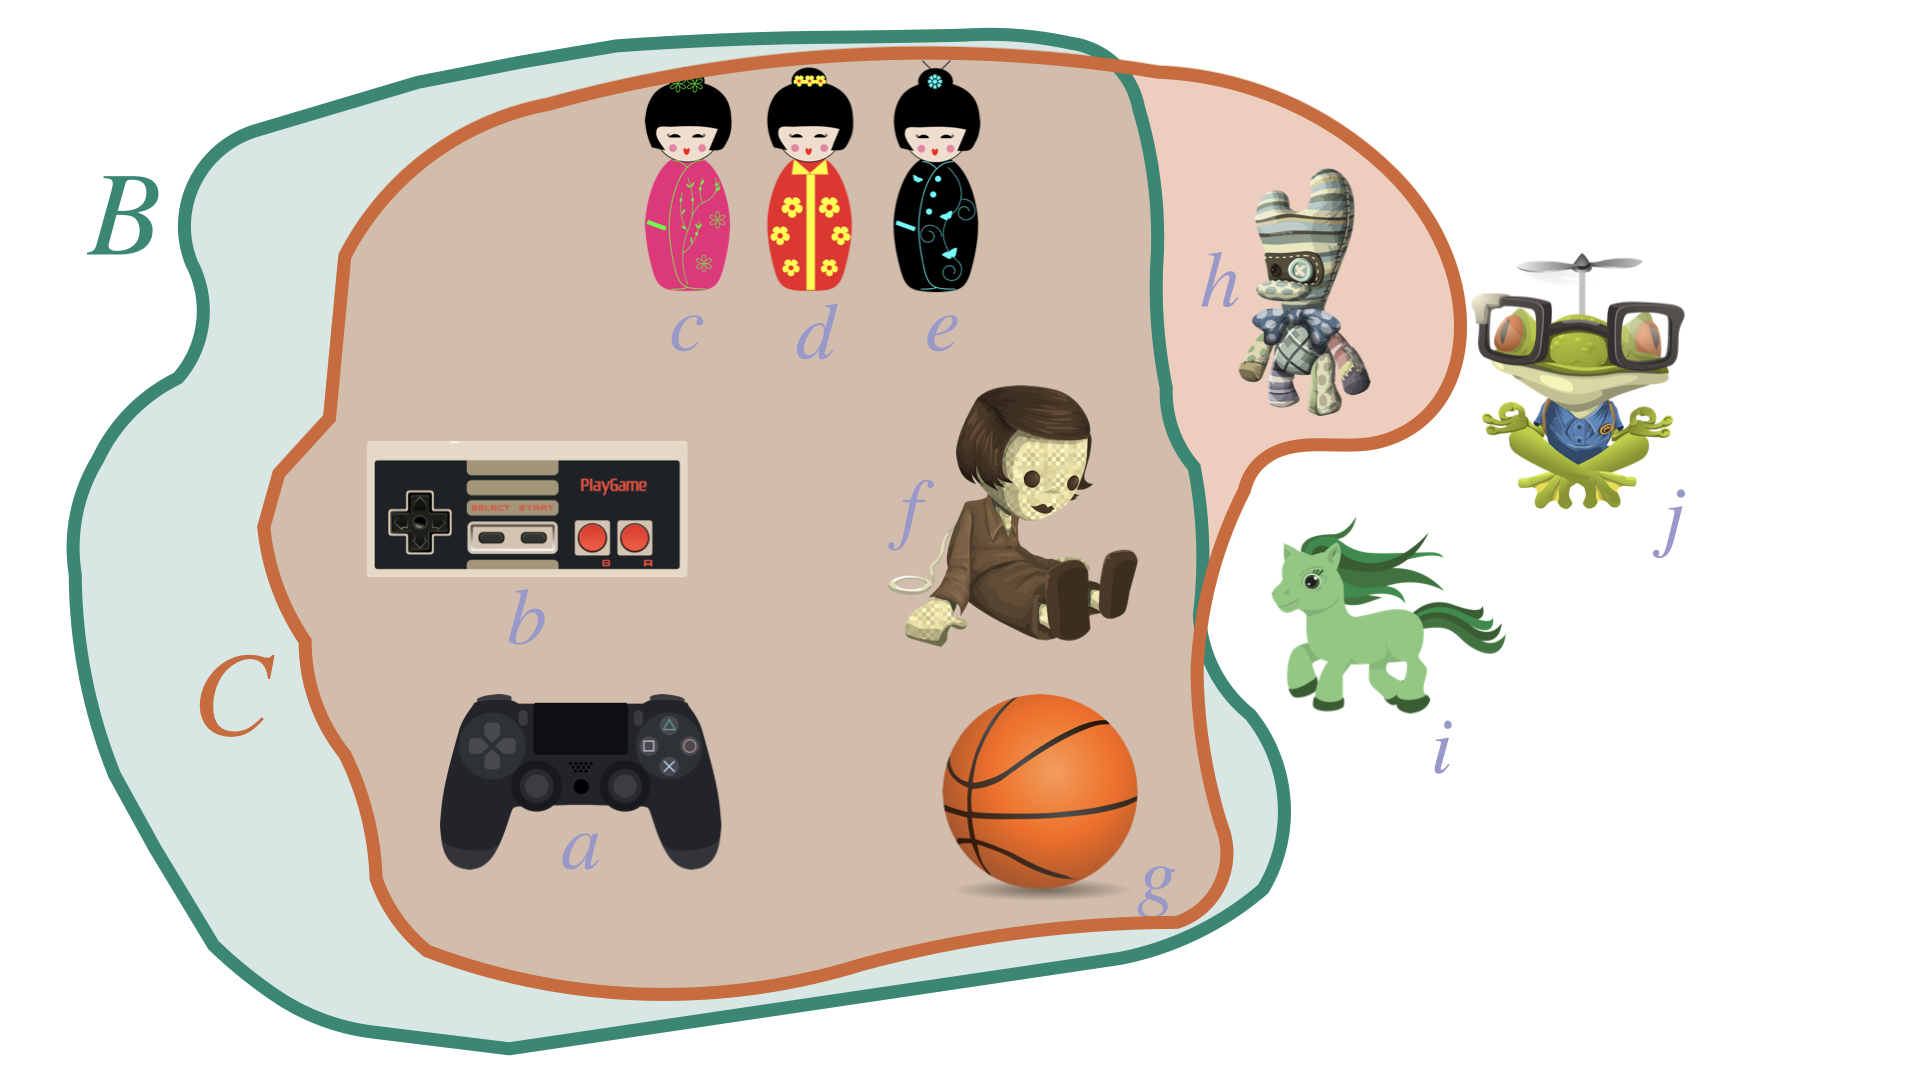
\includegraphics[width = 0.8\textwidth]{01b-sets-relations-operations/01b-sets-relations-operations-002.jpeg}

\end{frame}

\begin{frame}
  \frametitle{Example: Union}

  \hfill \textbf{Example 7: $B \cup C = \set{a, b , \dots, g, h}$}

  \bigskip

  \hfill 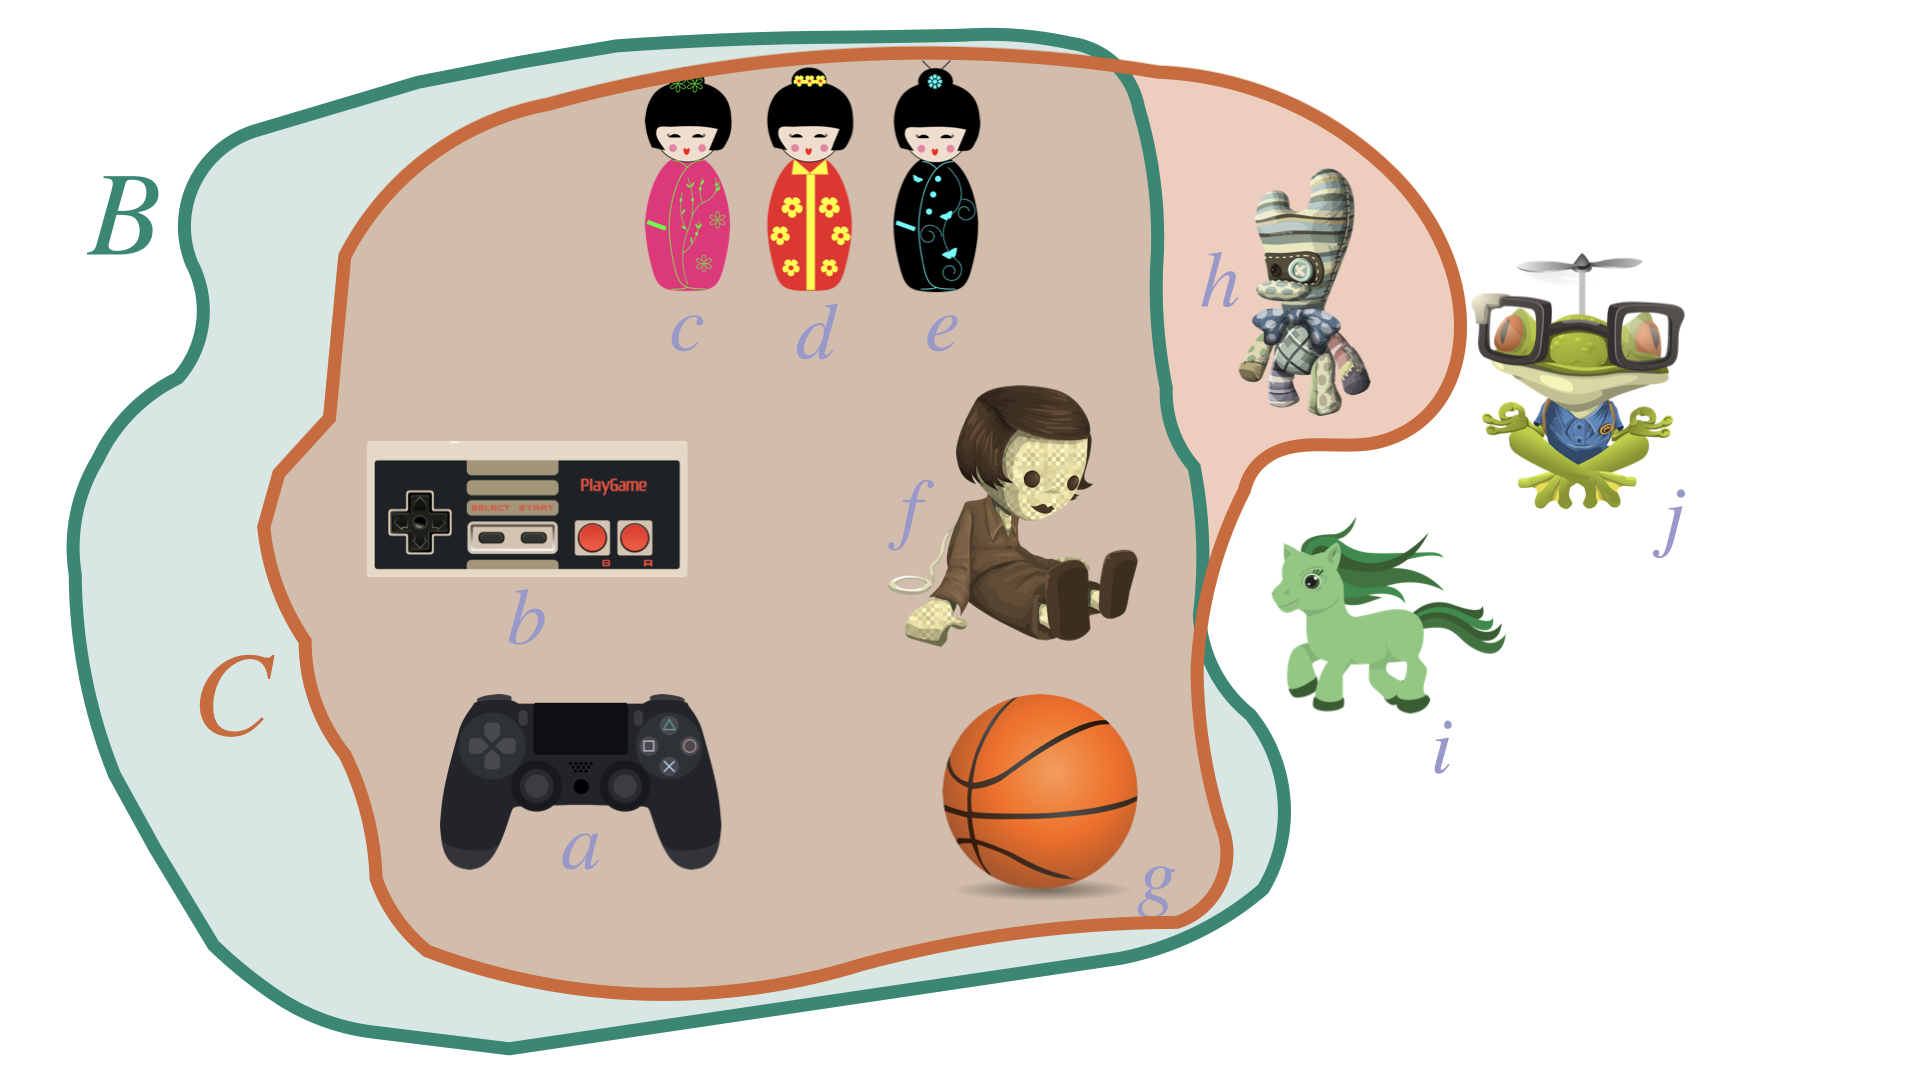
\includegraphics[width = 0.8\textwidth]{01b-sets-relations-operations/01b-sets-relations-operations-002.jpeg}

\end{frame}

\begin{frame}
  \frametitle{Example: Difference}

  \hfill \textbf{Example 8: $C \setminus B = \set{h}$ and $B \setminus C = \emptyset$} \\

  \bigskip

  \hfill 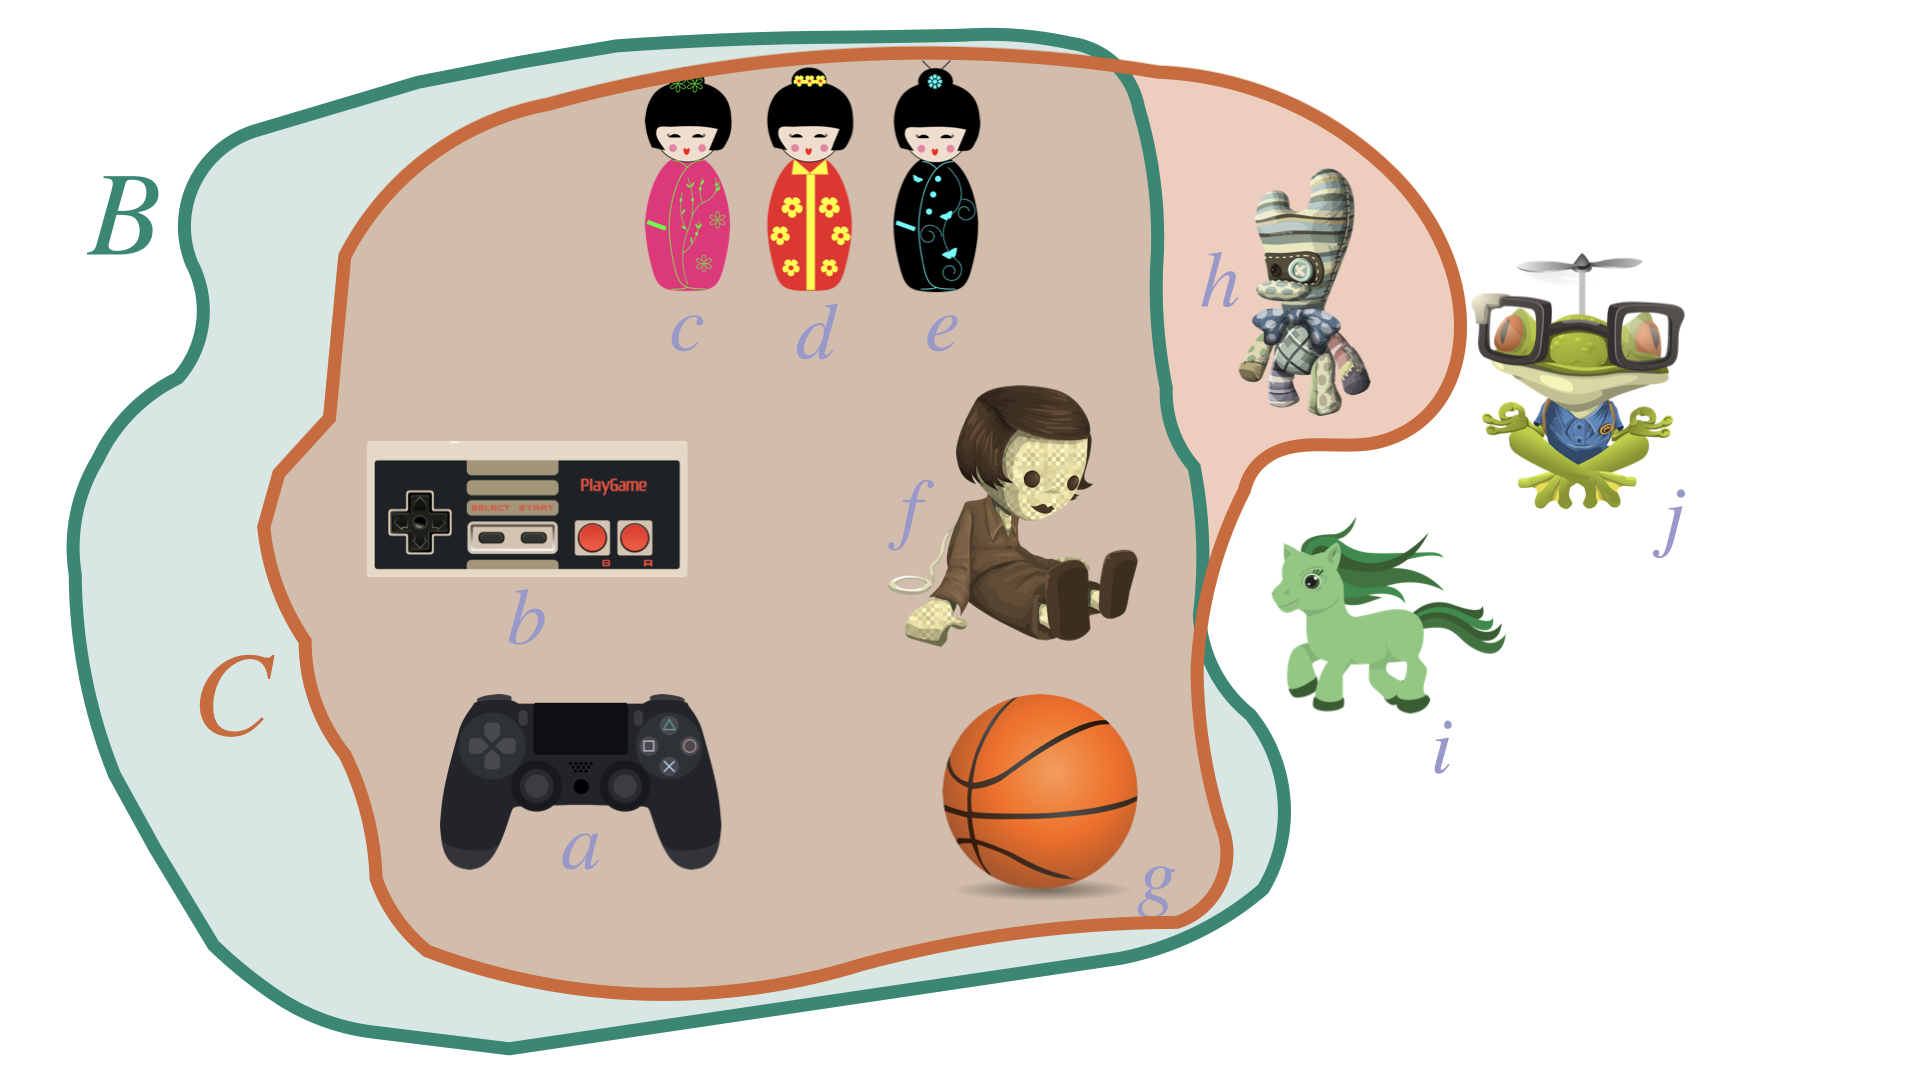
\includegraphics[width = 0.8\textwidth]{01b-sets-relations-operations/01b-sets-relations-operations-002.jpeg}

\end{frame}

\begin{frame}
  \frametitle{Example: Complement}

  \hfill \textbf{Example 9: $\overline{B} = \set{h, i , j}$ and $\overline{C} = \set{i,j}$} \\

  \bigskip

  \hfill 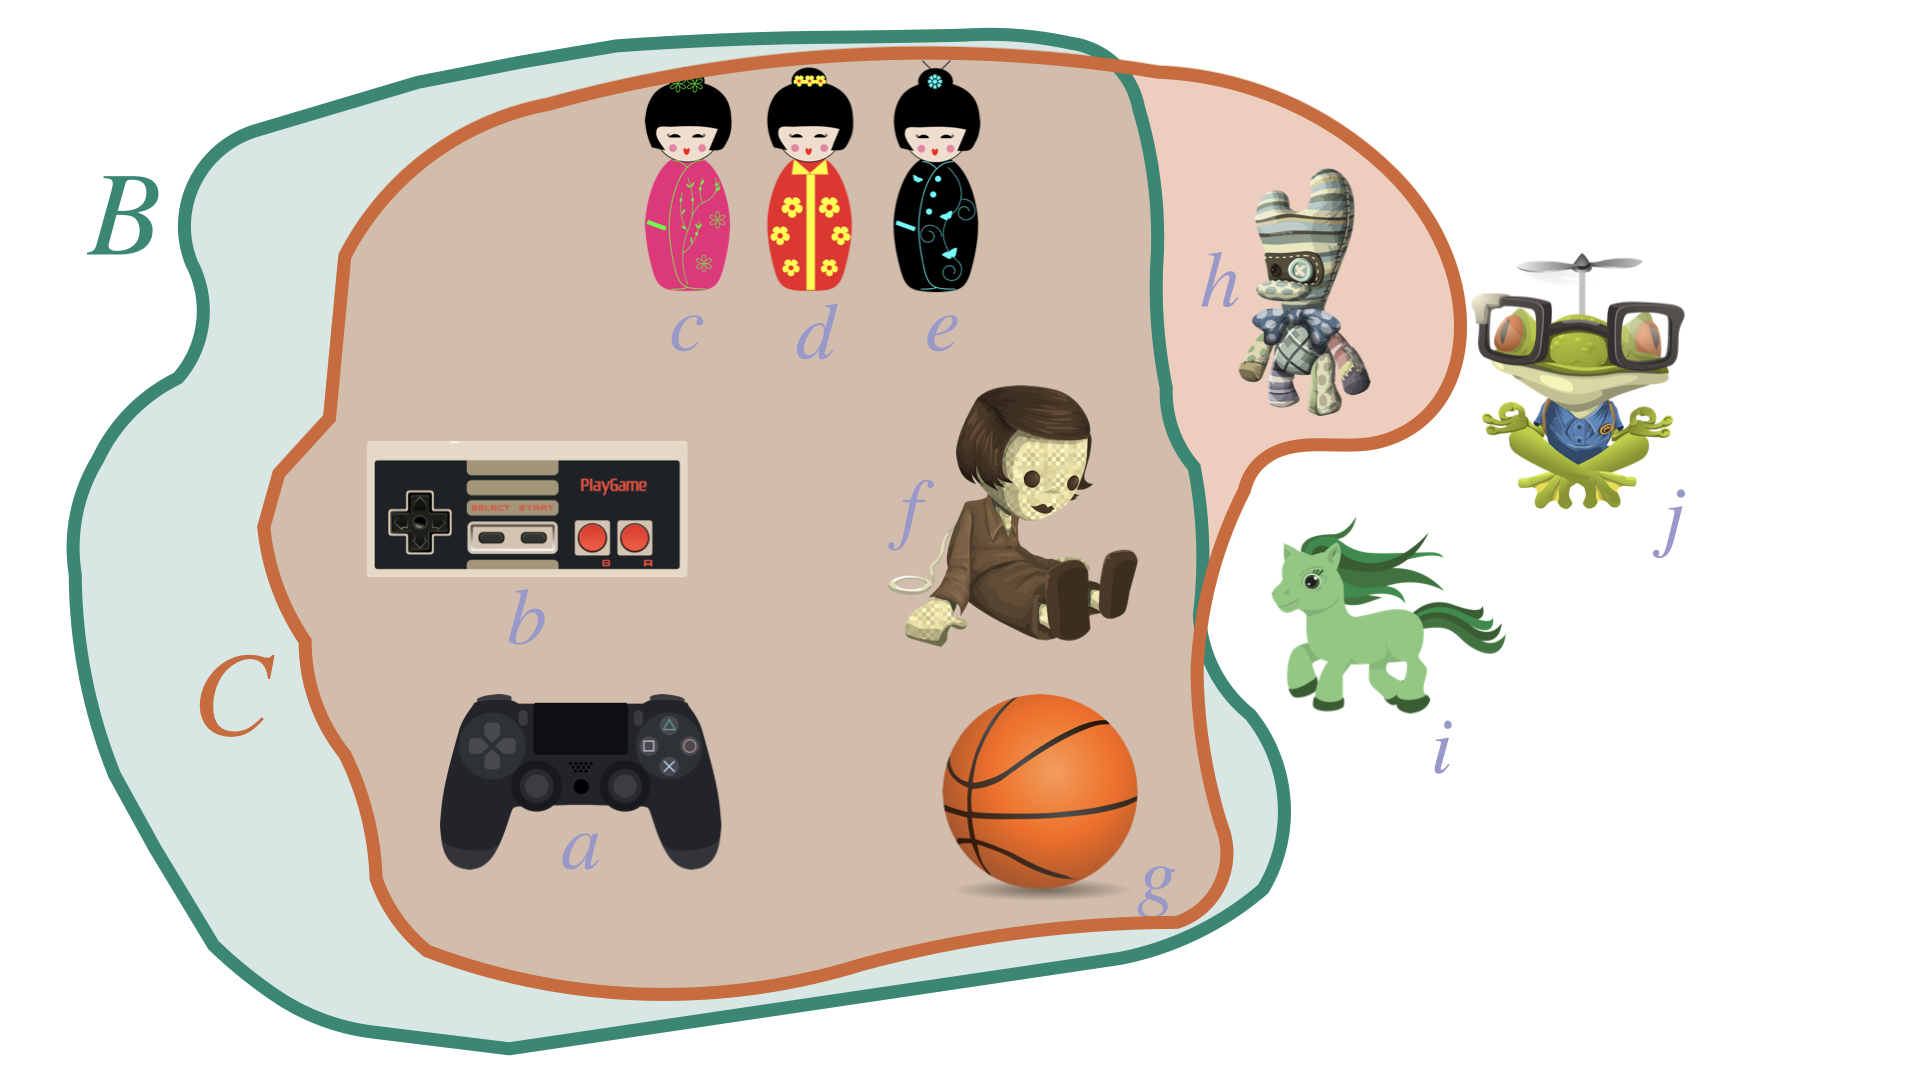
\includegraphics[width = 0.8\textwidth]{01b-sets-relations-operations/01b-sets-relations-operations-002.jpeg}

\end{frame}


\end{document}
